\documentclass[a0paper,portrait]{tikzposter}
\usepackage[T1]{fontenc}
\usepackage[utf8]{inputenc}
\usepackage[french]{babel}
\usepackage[backend=bibtex,doi=false,isbn=false,url=false]{biblatex}
\addbibresource{biblio.bib}
\usepackage{graphicx}

\usepackage{acronym}
\acrodef{mcs}[MCS]{simulation de Monte Carlo}

\title{Étude de Planning de taches par la simulation de Monte~Carlo.}   
\institute{Université de Strasbourg, laboratoire ICube UMR 7357, \\ 
Pôle API - 300 Bd Sébastien Brant - 67400 Illkirch-Graffenstaden - France} % See Section 4.1
\author{Luke Bertot}   
%\titlegraphic{Logo}
%\usetheme{default}  % See Section 5
\colorlet{backgroundcolor}{white}
\usetitlestyle{Wave}
\begin{document}
\maketitle  % See Section 4.1
\begin{columns}
  \column{0.65} \block{1.  Exécution d'application  de calcul  scientifique dans
    le Cloud}{%See Section 4.2
    Le Cloud permet  d'obtenir de la puissance de calcul  à la demande, avec un
    coût de location des ressources linéaire en le temps utilisé, compté en
    unités de temps (BTU). Comme toute plateforme mutualisée, on y observe une 
    variabilité des performances.\\

    Nous   avons   développé   un   système  de   courtage   de   cloud   appelé
    Schlouder~\cite{Michon2017}.  Schlouder ordonnance  l'exécution de jobs dans
    le cloud, se  charge du démarrage et  de l'extinction des VMs,  ainsi que de
    l'exécution  individuelle des  jobs. Schlouder  utilise des  stratégies pour
    déterminer combien de VMs démarrer et où placer les
    jobs. ASAP vise une exécution rapide, AFAP vise a minimiser les coûts.\\

    Nous  avons  exécuté  sur  un   cloud  privé  deux  application.  OMSSA  une
    application de protéomique  en bag-of-tasks et Montage est  un workflow pour
    la fusion d'image astronomiques. Pour  chaque exécution Schlouder relève les
    temps de démarrage,  les temps d'exécution de chaque jobs,  les coûts, et le
    temps total d'exécution.
    \\

Même sur un Cloud privatif comme le notre, on observe une variabilité
significative des temps d'exécutions. Cette variabilité est un obstacle aux
prédictions des coûts et du temps d'exécution total. La prise en compte de cette
variabilité requiert une simulation stochastique.\\

La Figure 1.\ ci-contre présente les distributions observées des temps d'exécution
(makespan) et des coûts (BTU count) pour chacune de ces applications. 
}
\column{0.35}
\block{}{%
	\begin{tikzfigure}[Distribtion du temps d'exécution et du coût dans la
		realité]
		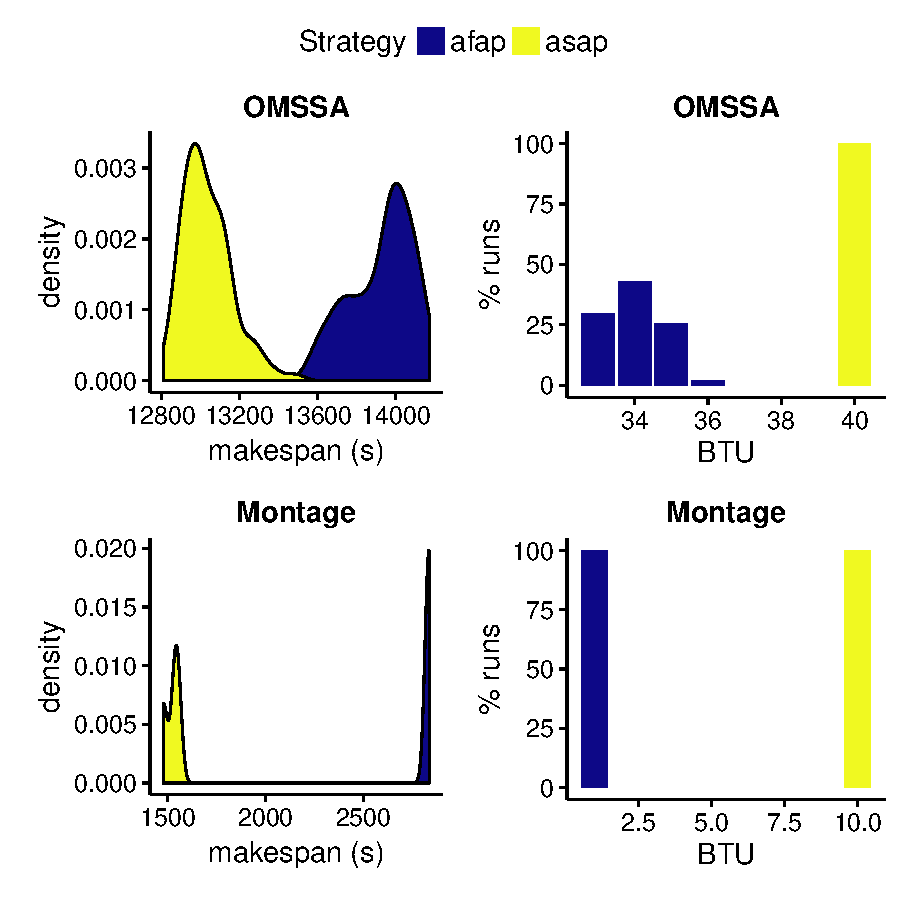
\includegraphics[width=0.97\linewidth]{gfx/real_plot.pdf}
	\end{tikzfigure}
}
\end{columns}


\begin{columns}  % See Section 4.4

\column{0.6}  % See Section 4.4

\block{2. Simulation de Monte Carlo}{%
\`A partir de SimGrid~\cite{simgrid}, nous avons développé une interface
permettant de modéliser les clouds IaaS. Avec cette interface, nous avons
pu développer SimSchlouder, un simulateur du courtier Schlouder.

Cependant, le moteur de simulation à évènements discrets de SimGrid est
déterministe et n'est pas adapté à la variabilité des temps d'exécutions et des coûts.\\

La \ac{mcs} permet de réaliser des simulations stochastiques
avec des simulateurs déterministes. Comme avec les méthodes de Monte Carlo dont 
elles découlent, les \ac{mcs} fonctionnent par tirage répété des valeurs aléatoires
pour échantillonner les résultats possibles.\\

Ici nos variables aléatoires d'entrée sont les temps d'exécution des jobs, et nos
variables de sortie le temps d'exécution total et le coût.\\
\begin{tikzfigure}[Simulation de Monte Carlo]
	\begin{tikzpicture}[
sim/.style={%
draw, 
rounded corners
}
]
%% Origin node
\node[align=center]at(0,2){Job\\RVs};
\node at(0,0)(orig){$\{R_1,\ldots,R_n\}$};
%% Realisations
\node at(3.5,2){Realisations};
\node[]at(3.5,1)(pert1){$\{T_1^1,\ldots,T_n^1\}$};
\node at(3.5,0){\vdots};
\node at(3.5,-1)(pert5){$\{T_1^{500},\ldots,T_n^{500}\}$};
\draw[-{latex}](orig)--(pert1);
\draw[-{latex}](orig)--(pert5);
%%
\node[sim]at(6,1)(s1){Sim};
\node[sim]at(6,-1)(s5){Sim};
\node at(6,0){\vdots};
\draw[-{latex}](pert1)--(s1);
\draw[-{latex}](pert5)--(s5);
%% Makespans
\node at(8,2){Samples};
\node at(8,1)(M1){$M^1$};
\node at(8,-1)(M5){$M^{500}$};
\node at(8,-0){\vdots};
\draw[-{latex}](s1)--(M1);
\draw[-{latex}](s5)--(M5);
%% Consolidation
\node[align=center]at(10,2){Makespan\\RV};
\node at(10,0)(r){$M_S$};
\draw[-{latex}](M1)--(r);
\draw[-{latex}](M5)--(r);
%%phases
\node[align=center]at(1.75,-2.5)(df){realisation\\draw};
\draw[dotted](1.75,1.5)--(1.75,-2);
\node[align=center]at(9,-2.5)(df){distribution\\fitting};
\draw[dotted](9,1.5)--(9,-2);
\end{tikzpicture}

\end{tikzfigure}
}
\block{4. Résultats}{%
La Figue 3.\ ci-contre, présente la distribution des résultat des simulations
d'une MCS et les compare à la réalité (en bleu). Notre MCS capture une très grande
partie des exécutions réelles.

Lorsque l'on agrège les temps d'exécution obtenus par les simulations avec une
loi normale, les intervalles de confiance à 99\% obtenus capturent 100\% des cas
réels, à l'exception de OMSSA/ASAP où le taux de capture et de 98\%. 

Du coté du coût, la simulation capture toutes les possibilités de nombres de BTU
possibles pour un couple application/stratégie donnée.\\

Néanmoins notre modèle est trop simpliste pour capturer exactement la 
distribution des temps d'exécution et des coûts. Dans la réalité la variabilité
des temps d'exécution n'est pas uniforme et change de job à job.
}
\block{5. En Résumé}{%
Le Cloud présente un variablité inhérente qui affecte le coût et le temps
nécessaire à l'exécution d'une application. Cette variabilité est un frein à
l'usage de la simulation comme outil de prédiction.\\

La simulation de Monte Carlo nous permet de modéliser la variabilité
d'une application exécutée sur le cloud avec une précision suffisante pour
fournir un intervalle de confiance du temps total d'exécution et du coût.
}
\column{0.4}
\block{3. Modèle Applicatif}{%
Pour modéliser la variabilité des jobs sur notre plateforme de cloud on considère
chaque temps d'exécution comme étant une base fixe auquelle est appliquée une
perturbation tirée aléatoirement. \[T_i^n = T_i * (1+r)\] 
avec $T_i$ le temps moyen observé pour le job $i$, et $r$ une valeur aléatoire
obtenue par un tirage uniforme dans l'intervalle $[-P,+P]$.\\

Le niveau de perturbation $P$ est global pour toute la \ac{mcs} et est défini
comme étant la moyenne des plus grands écarts à la moyenne observée. 
Pour notre Cloud ce niveau de perturbation est de 10\%.
} 
\block{}{%
\begin{tikzfigure}[Distribution des temps d'éxecution et des coûts obtenus par
la MCS]
	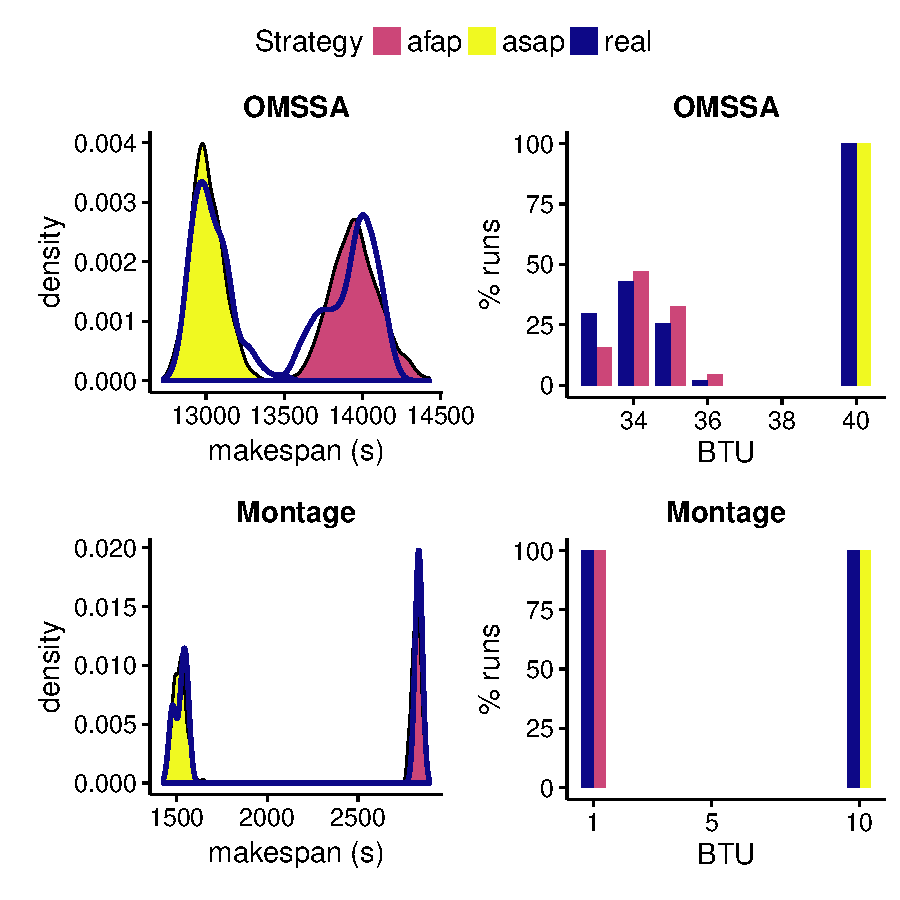
\includegraphics[width=0.9\linewidth]{gfx/fit_plot.pdf}
\end{tikzfigure}
}
\block{Références}{\printbibliography[heading=none]}
\end{columns}

\end{document}
% vim:spell spelllang=fr:
